%************************************************
\chapter{Esempi e applicazioni}\label{cap:esempi}
%************************************************

In questo capitolo mostreremo alcuni esempi con dati sintetici che mostrano il tipo di visualizzazione che si riesce ad ottenere utilizzando l'omologia persistente, poi vedremo come la TDA è stata usata in diversi studi per ricostruire la struttura da un insieme di \emph{patch} ad alto contrasto estratti da immagini naturali.

\section{Esempi in basse dimensioni}

Come primi esempi mostriamo in \cref{fig:examplecirclesbarcodes} i codici a barre persistenti rispettivamente di un cerchio nel piano e di due cerchi nel piano.

\begin{figure}[h]
  \caption{Esempi di codici a barre persistenti}
  \label{fig:examplecirclesbarcodes}
  \centering
  \includegraphics[width=.8\linewidth]{gfx/circle_persistence.pdf}
  \subcaption{Estrazione casuale da un singolo cerchio}
  \centering
  \includegraphics[width=.8\linewidth]{gfx/two_circles.pdf}
  \subcaption{Estrazione casuale da due cerchi}
\end{figure}

Anche in questi casi banali è possibile osservare come la diversa distribuzione dei punti sui cerchi causa interssanti artefatti, come si può osservare dall'omologia persistente 0-dimensionale nel caso dei due cerchi, in cui la presenza di due componenti connesse non è così marcatamente evidente dal codice a barre persistente.

(NMDC: aggiungere toro e sfera)

\section{Struttura dell'insieme delle patch $3\times 3$ in una collezione di immagini naturali}

In questa sezione ripercorreremo lo studio omologico di un insieme di costruito da
Lee, Pedersen e Mumford in \cite{Lee2003} e analizzato in \cite{Carlsson2008} e \cite{DeSilva2004}.

L'insieme di dati è composto da immagini in bianco e nero, catturate mediante una fotocamera digitale, e si può pensare a ciascuna di queste immagini come a un vettore di pixel in uno spazio vettoriale di dimensione estremamente alta, e dove la coordinata corrispondente a un certo pixel è il valore nella scala di grigi di quel pixel.

\begin{figure}[ht]
  \begin{center}
    \includegraphics[width=.8\linewidth]{gfx/example_patches.pdf}
    \caption{Esempi di patch $3\times 3$ ad alto contrasto}
    \label{fig:examplepatches}
  \end{center}
\end{figure}

Poiché la dimensione di questo problema è estremamente elevate è impossibile pensare di analizzare direttamente direttamente questo insieme, tuttavia si può studiare il problema di dimensione più ridotta di studiare la statistica delle piccole patch (blocchi $3\times 3$ estratti dalle immagini) ad alto contrasto, come quelle in \cref{fig:examplepatches}.

Detto $\mathcal{M}$ l'insieme di immagini che si vuole sturiare, il procedimento che porta a selezionare le patch su cui viene effettuata l'anlisi è il seguente:
\begin{enumerate}
  \item Da ogni immagine di $\mathcal{M}$ vengono estratte casualmente un numero $L$ elevato di patch $3\times 3$. Tutte queste patch vengono considerate come un sottinsieme $\mathcal{P}_1$ di $\R^9$.
  \item Ogni $x\in\mathcal{P}$ viene riscalato in $\tilde{x}$ con $\tilde{x}_i = log(x_i)$.
  \item Per ogni vettore $\tilde{x}$ si calcola il suo contrasto (detto anche $D$-norma) $\normD{\tilde{x}}=\sqrt{\tilde{x}^\mathbf{T}D\tilde{x}}$, dove $D$ è una forma bilineare che tiene conto della differenza di ciascun pixel della patch con quelli adiacenti e definita nel seguente modo: scriviamo $i\sim j$ se i pixel corrispondenti all'$i$-ma e $j$-ma coordinata rispettivamente sono adiacenti, e definiamo
  \begin{equation*}
    \normD{x} = \sqrt{\sum_{i\sim j}(x_i-x_j)^2}.
  \end{equation*}
  \item Si conserva solo il $20\%$ delle patch con $D$-norma più alta.
  \item Si sottrae a ogni $\tilde{x}$ la sua media $\mu(x)=\displaystyle\frac{1}{9}\sum_{i=1}^9\,x_i$, in modo che i nuovi punti $\tilde{y}$ si trovino sull'iperpiano $H\subseteq\R^9$ definito da $\sum_{i=1}^9 x_i =0$.
  \item Si normalizza ciascun vettore dividendolo per la sua $D$-norma.
\end{enumerate}

I dati così elaborati si trovano adesso su un ellissoide $S^7\subseteq\R^9$, indichiamo con $\widetilde{\mathcal{M}}$ l'insieme delle patch rinormalizzate. Nel caso analizzato in \cite{Lee2003} e \cite{Carlsson2008} l'insieme è costituito da $4.5 \times 10^6$ patch.

Come è stato fatto nella \cref{sec:functionalpersistence} vogliamo filtrare i dati per densità. Questa volta useremo come funzione di densità $e_k$ con $k$ intero positivo, dove $e_k(x)$ è la distanza di $x$ dal $k$-mo punto di $\widetilde{\mathcal{M}}$ più vicino a $x$. Poiché $e_k$ è una misura inversa di densità, siamo interessati a punti che abbiano $e_k$ piccolo. Questo giustifica la seguente definizione.

\begin{definition}
  Dato un intero $k$ e una percentuale $p$, definiamo il sottinsieme $X(k,p)\subseteq\widetilde{\mathcal{M}}$ come il $p\%$ più piccolo secondo $e_k$.
\end{definition}

A questo punto possiamo studiare al variare dei parametri $k$ e $p$ le proprietà topologiche di $X(k,p)$. Per $k$ grande i dati si dispongono essenzialmente in cerchio, come mostrato dal diagramma di persistenza \cref{fig:k300persistence} tratto da \cite{Carlsson2008}.

\begin{figure}[ht]
  \begin{center}
    \includegraphics[width=.8\linewidth]{gfx/image_patches_k300.pdf}
    \caption{L'omologia persistente di $X(300,30)$}
    \label{fig:k300persistence}
  \end{center}
\end{figure}

In \cite{Carlsson2008} e \cite{DeSilva2004} viene mostrato come sia possibile parametrizzare i dati così selezionati in un cerchio, detto primario. In \cref{fig:primarycircle} lo vediamo rappresentato insieme alle patch che lo compongono.

% TODO draw primary circle
\begin{figure}[ht]
  \begin{center}
    \includegraphics[width=.4\linewidth]{gfx/primarycircle_labels.pdf}
    \caption{Le patch sul cerchio primario}
    \label{fig:primarycircle}
  \end{center}
\end{figure}

Se scegliamo un parametro $k$ più piccolo (e quindi selezioniamo punti più densi) vengono scoperte nuove strutture, come si vede dall'omologia persistente di $X(15,30)$ in \cref{fig:k15persistence} (presa da \cite{Carlsson2008}).

\begin{figure}[ht]
  \begin{center}
    \includegraphics[width=.8\linewidth]{gfx/image_patches_k15.pdf}
    \caption{L'omologia persistente di $X(15,30)$}
    \label{fig:k15persistence}
  \end{center}
\end{figure}

Vi sono diversi spazi topologici che hanno questa omologia, e cioé connessi con primo numero di Betti $\beta_1=5$, ad esempio lo spazio mostrato in \cref{fig:patchshape}. In \cite{Carlsson2008} viene data una parametrizzazione dei dati mediante uno spazio di polinomi, e con questi è possibile vedere che la forma rappresentate in \cref{fig:patchshape} è effettivamente corretta.

\begin{figure}[ht]
  \begin{center}
    \includegraphics[width=.4\linewidth]{gfx/patches_shape_labels.pdf}
    \caption{La struttura a tre cerchi $C_3$}
    \label{fig:patchshape}
  \end{center}
\end{figure}

Possiamo anche visualizzare le patch corrispondenti ai due nuovi cerchi (detti secondari), in \cref{fig:secondarycircle}

\begin{figure}[ht]
  \begin{center}
    \includegraphics[width=.8\linewidth]{gfx/secondarycircles.pdf}
    \caption{Le patch sui cerchi secondari}
    \label{fig:secondarycircle}
  \end{center}
\end{figure}

Infine, $X(15,30)$ è contenuto in un insieme di patch che forma una bottiglia di Klein, in \cref{fig:kleinpatch} vediamo come si dispongono i cerchi principali e secondari sulla bottoglia di Klein e come variano le patch.

\begin{figure}[ht]
  \begin{center}
    \includegraphics[width=.6\linewidth]{gfx/kleinpatches.pdf}
    \caption{Immersione di $C_3$ nella bottiglia di klein}
    \label{fig:kleinpatch}
  \end{center}
\end{figure}
